\subsection{Zero Degree Calorimeter}

The ATLAS Zero Degree Calorimeter (ZDC) is designed to detect neutral particles that very close to the beampipe. It consists of two detectors located in absorbers along the beamline $\pm 140$ m from the ATLAS interaction point. Each side (or arm) consists of four modules each with a material budet of 1.14 hadronic interaction lengths.  The sampling calorimeter design consists of insterspered absorber layers, which cause the incident particles to shower, and active layers, which output a signal proportinal to the energy deposited by charged particle shower crossing that layer.  The absorber layers consist of tungstan plates, and the active layers consist of cherenkov radiators.  These Cherenkov radiators transport Cherenkov radiation\footnote{Cherenkov radiation is emmited in a mach cone when paerticles travel faster than the local speed of light in the material medium} induced by the particle shower to the lens of a Photomultiplier tupe (PMT).  Each of the four modules are instamented with a single PMT.  Cherenkov radiators were chosen since they offer substantial radiation hardness, quite necessary for a location that recives a very high dose.  In Run 2, the active layers consisted of Quartz rods as the active layer.  The radiation hardness of the deterctor was improved considerably in Run 3 when the active layer was replaced with doped fused silica rods.

As a calorimeter, the ZDC destructively samples the energy of the particles that enter it.  Since dipole magnets between the IP and the ZDC swipe away forward charged particles, only neutral particles enter the ZDC.  In ion running, the fragmentation of the ion's nucleus results in a population of neutrons interacting in the ZDC.  Since these so called "spectator" neutrons do not interact in the collision at the IP they will impact the ZDC with roughly the same per nucleon energy as the beam.  The number of spectator neutrons in non-trivially dependent on the event geometry, but they range from zero to roughly $(A-Z)/2$.

In order to capture signals from a zero to many neutrons, the ZDC operates with two sets of readout instrumentation, denoted as high and low gain readouts.  The high gain readout is configured to have a dynamic range that saturates with a couple of neutrons.  The low gain readout has a range of a roughly 10x that of the high gain readout.
%Each readout consisted of two 40 MHz ADCs (25 ns).  Both ADCs read out the same signal, but one is delayed by 12.5 ns.  This allows for the combined readout to have a sampling of 80 MHz (12.5 ns).

The ZDC reconstruction software transforms the raw data read out from the above ADCs into module specific amplitures.
Firstly, each waveform must have its pedestal subtracted in order to make sure that the output amplitude represents only strength of the module signal and not any offset caused by the electronics configuration.  Then, the subtracted samples can be fit to a functional waveform.  The amplitude that minimize the $\chi^2$ of this fit is then considered to be the aplitude in that given event.
\TCR{Prob need to include more details about the ZDC reconstruction}

Finally, the ZDC calibration transforms the above amplitudes, which have units of ADC counts, into units of energy.

\paragraph{Missing ZDC Module in 2016 Data}
\label{sec:missing_zdc_mod}
During the 2016 \pxPb\ run, the ZDC side C module 0 (EM) was removed and replaced with the Arm2 calorimeter of the LHCf experiment~\cite{Adriani:2135330}. Figure~\ref{fig:lhcf_v_zdc_acceptance} displays the transverse acceptance of both the ATLAS ZDC and LHCf. The ATLAS ZDC EM module is the first of four sequential calorimeter modules, counting from the perspective of looking at the ZDCs from the ATLAS interaction point; therefore, the LHCf calorimeter would see forward neutral products before they reach the side C ZDC. The LHCf detector was put in place to measure the forward neutral products of the proton-going side in the \textbf{Period B} orientation; however, in the \textbf{Period C} orientation the LHCf detector was retracted into the ``garage'' position to avoid radiation damage~\cite{Adriani:2135330}. The ``garage'' position indicates an upward vertical shift of 112~mm from the nominal position shown in Figure~\ref{fig:lhcf_v_zdc_acceptance}. This shift places the full LHCf Arm2 calorimeter outside of the full acceptance of the ATLAS ZDC. The side C ZDC has roughly 75\% of the material budget of side A. This effectively reduces the interaction length of the side C ZDC from 4.6 to 3.4, which in turn reduces the neutrons expected to shower in the ZDC from 99\% to 96.6\%.

\begin{figure}[p]
    \centering
    \begin{subfigure}[c]{0.42\linewidth}
        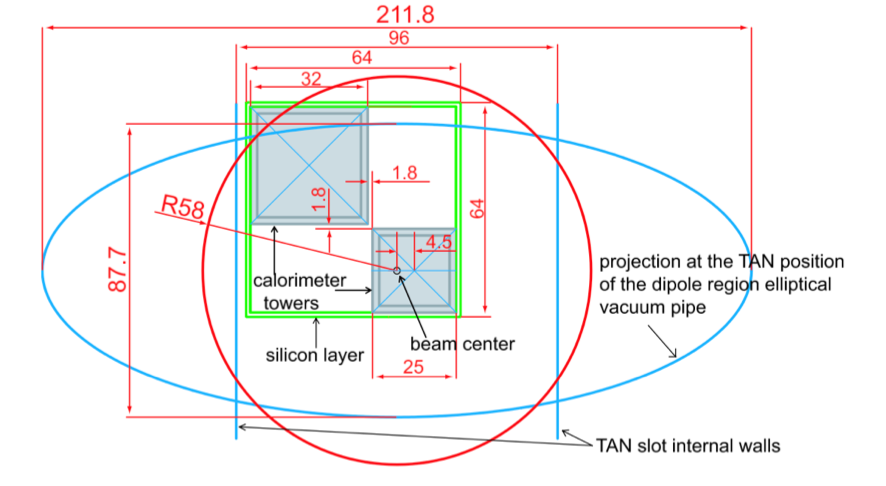
\includegraphics[
            width=1\linewidth,
            alt={Transverse acceptance of the LHCf Arm2 calorimeter viewed from the ATLAS interaction point.}
        ]{chapters/geometry_estimators_pPb/figures/dataset_and_event_selection/lhcfAcceptence.png}
    \end{subfigure}
    \begin{subfigure}[c]{0.42\linewidth}
        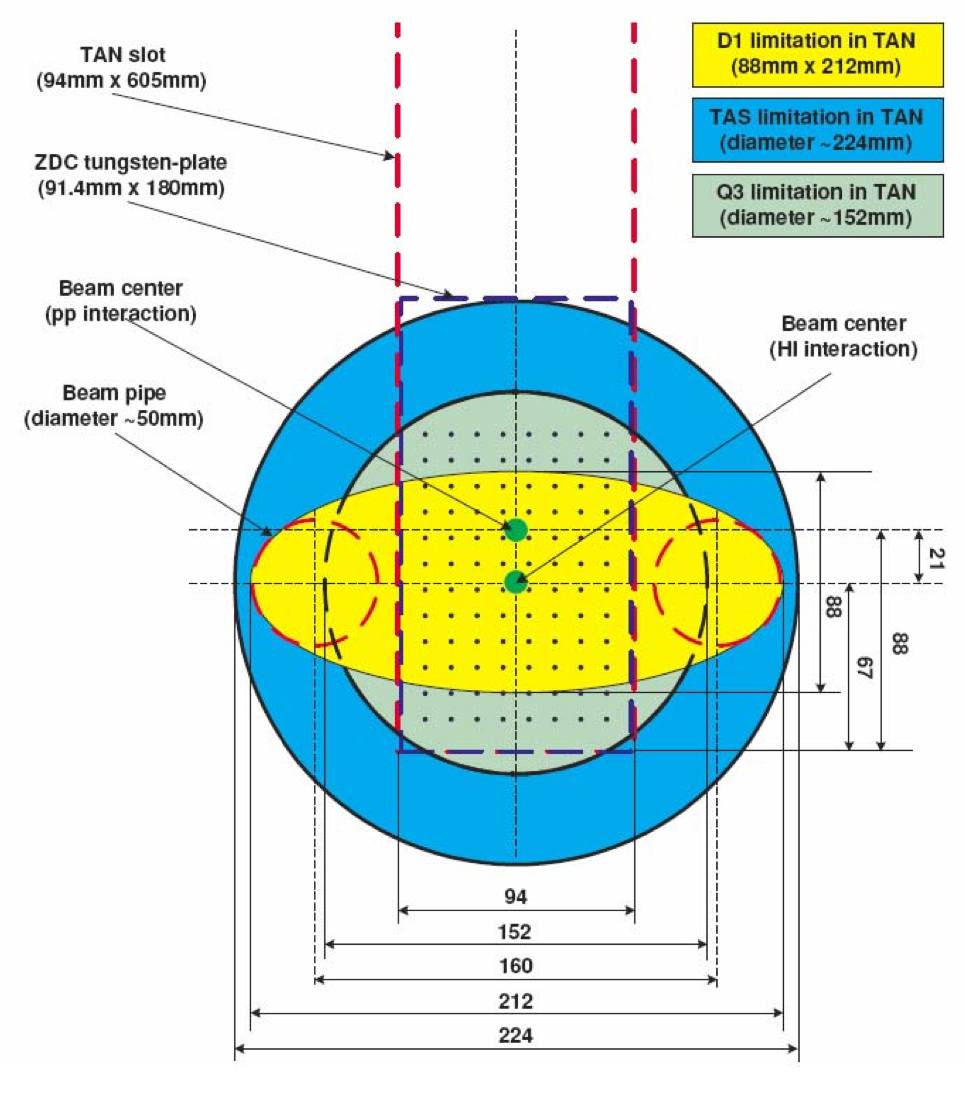
\includegraphics[
            width=1\linewidth,
            alt={Transverse acceptance of the ATLAS ZDC viewed from the ATLAS interaction point.}
        ]{chapters/geometry_estimators_pPb/figures/dataset_and_event_selection/zdcAcceptence.png}
    \end{subfigure}
    \caption{Detector geometry for LHCf Arm2~\cite{Cekmecelioglu:2867369} (left) and the ATLAS ZDC~\cite{Jenni:1009649} (right), viewed from the ATLAS interaction point. Distances are given in mm. The blue oval in the left image corresponds to the boundary of the yellow oval in the right image. The active area of LHCf is represented by the filled blue squares, and the active area of the ZDC is bounded by the purple dashed line.}
    \label{fig:lhcf_v_zdc_acceptance}
\end{figure}

\FloatBarrier
\subsubsection{2016 \texorpdfstring{$p$}{p}+Pb ZDC Calibration}

Due to the asymmetric nature of the \pxPb\ collisions system in each period only one arm of the ZDC detector will recive ion fragments.

In 2019, J. Nagle performed \TCR{ ref needed} the calibration of the 5.02 \TeV\ data, but concluded that the contamination from pileup in the high-\avmu\ \pxPb\ data made a calibration unfeasible.

The author of this thesis undertook the calibratrion of the high high-\avmu\ \pxPb\ data in 2023 after substatial improvemnts had been made to the ZDC reconstruction in order to mitigate the previously untennable issues.

The first improvement made to the ZDC reconstruction comes from \cite{ATL-COM-PHYS-2019-1454}.  This note documents updates to the signal processing created mainly for the 2018 \PbxPb\ data, but that are useful for the 2016 \pxPb\ data as well.  These updates includes significant improvements to the reconstructions ability to fit pulses in the presence of out of time (OOT) pile up, both preceding and after the event in question.  Large OOT pileup pulses would saturate the high gain ADC, leading to the pulse being analyzed with the low gain ADC which has a roughly 10x worse resolution.  By excluding a few samples from the beginning or (end) of these pulses and looking at the high gain ADC values, the reconstruction will yield a reasonable fit for the current event. This is especially important given that the relatively high \avmu\ in the 2016 8.16 \TeV\ \pxPb\ has more events affected by out of time pileup.

The second significant improvement made to the ZDC reconstruction was the `two-pass' analysis method.  This method first uses a relatively high second derivative threshold to search for pulses in a ZDC event.  This high threshold helps to suppress noise from small background and pileup pulses.  However, if at least one module has a pulse that passes this threshold, all the modules on said ZDC arm are reanalyzed with a lower second derivative threshold. This `repass' recovers finer pulses that were too small to be `seen' on the first pass.

The third significant improvemnt\footnote{This improvment was done by the author of the thesis, while the first two were done by Pengqi Yin of Columbia University}, involves the studies on the pulse timing.

\begin{figure}[ht]
    \centering
    \includegraphics[width=.55\linewidth]{chapters/the_lhc_and_atlas/figures/zdc_detector/T0plot1.pdf}
    \caption{Example of a fitted ZDC pulse, taken from \cite{ATL-COM-PHYS-2019-1454} }
    \label{fig:pulse}
\end{figure}

Base ZDC pulses (see Figure~\ref{fig:pulse}) are fit to a function of the form given in Equation~\ref{eqn:fermiexp}, hereafter referred to as a FermiExp pulse.

\begin{equation}
    \label{eqn:fermiexp}
    f(t\mid A,\tau_1,\tau_2,t_0,C) = A \left( \frac{e^{-(t-t_0)/\tau_2}}{1+e^{-(t-t_0)/\tau_1}} \right)+C
\end{equation}

Several of these parameters are fixed in order for the fitting function to have fewer degrees of freedom and thus converge more efficiently.  For example, $\tau_1\ \&\ \tau_2$ are fixed in the 2016 ZDC reconstruction.

From a data quality standpoint, it would be useful to be able to reject pulses that were relatively early or late when compared to other pulses. One way to do this would be by defining a nominal $t_0$ range that is acceptable.  However, there are two main challenges to defining a nominal $t_0$.
\begin{enumerate}
    \item When the high voltage powering the a ZDC PMT changes, it affects the transit time in the tube which leads to a slightly different nominal $t_0$. \newline \textbf{Solution:} Implement a time dependent nominal $t_0$ correction for the entire dataset.
    \item There is a nonlinear dependence of the $t_0$ on the pulse amplitude that must be corrected.  \newline \textbf{Solution:} Fit the curvature induced by the nonlinear dependence to a 5th order polynomial.  Use that fit function to flatten the convex distribution.
\end{enumerate}

The data used for the calibration of the high-\avmu\ \pxPb\ was read out into a dedicated ZDC calibration stream.  This dedicated readout only stores information about the ZDC detector for each accepted event\footnote{The per-event data footprint of the ZDC detector is roughly an order of magnitude smaller than the whole ATLAS detector including all detector subsystems} and can therefore accumulate substantial statistics needed for a precision calibration.  Events entereing the stream fired the \triga~or~\trigc\ triggers, requiring that there was some substatial energy in at least one arm of the ZDC.  To get a set of events unbiased by trigger turn on thresholds, the set of events used to analyze Side A were triggered on a signal in Side C and vice versa.

The ZDC is designed to sample neutral ion fragments with the same per-nucelon energy as the beam.  The lightest neutral fragment possible is a single beam energy neutron incident on the detector.  A single neutron that fragmented from a lead ion will, on average, be as energetic as the per-nucleon beam energy, which here is 2.5625~\TeV.  Therefore, the energy of single neutrons gives a well defined energy to calibrate against.  Of course single neutrons will not have the exact per-nucleon beam energy every time, since the exact energy of bonud nucleons is stochastically modified by the so-called `fermi-momentum'~\TCR{citation needed}.  The variance of single neutrons given by fermi-momentum coupled with the experimental resolution of the ZDC should give the width of the detector response to a single neutron.

Therefore the single neutron peak~\footnote{observed detector response to single neutrons} intrinsically contains information about the ZDC Energy Scale ($\mu_{\mathrm{1n}}$) and ZDC Energy Resolution ($\sigma_{\mathrm{1n}}$).  However, we are intereted in not just any calibration, but the \textit{optimal} one. The optimal calibration is defined to be the one that puts the mean of the single neutron peak at 2.5625~\TeV\ and minimizes the variance (therefore maximizing experimental resolution).  The machinery of the calibraiton works as follows.

The goal is to find a set of gains $\mathbf{g} = \{g_0,g_1,g_2,g_3\}$ such that given the ZDC module amplitudes for a given event $\mathbf{A} = \{A_0,A_1,A_2,A_3\}$ the dot product $\mathbf{g}^T\mathbf{A}$ is equal to the energy of the ZDC in units of \GeV (2562.5 \GeV).  The below calibration procedure is performed on a subset of ZDC events in the first neutron peak.  Equations~\ref{1nmean}~and~\ref{1nvar} are the mean an variance of the first neutron peak sample. The variable $N$ indicates the size of the sample used to perform the analysis.
\begin{equation}
    \label{1nmean}
    E_{\text{1n}} = \bigl \langle \mathbf{g}^T\mathbf{A} \bigr \rangle_{N}
\end{equation}
\begin{equation}
    \label{1nvar}
    \sigma^2 = \Bigl \langle \left( \mathbf{g}^T\mathbf{A} \right)^2  \Bigr \rangle_{N} - \left( \bigl \langle  \mathbf{g}^T\mathbf{A}  \bigr \rangle_{N} \right)^2 = \Bigl \langle \left( \mathbf{g}^T\mathbf{A} \right)^2  \Bigr \rangle_{N} - \left( \text{E}_{\text{1n}} \right)^2
\end{equation}
Using the method of Lagrange multipliers, one can minimize the variance under the constraint that mean of the one neutron peak is equal to the per nucleon beam energy.
\begin{equation}
    \label{LagrangeMult}
    \mathcal{L} = \Bigl \langle \left( \mathbf{g}^T\mathbf{A} \right)^2  \Bigr \rangle_{\text{N}} - \left( \text{E}_{\text{1n}} \right)^2 + \lambda\left( \bigl \langle \mathbf{g}^T\mathbf{A} \bigr \rangle_{\text{N}} -  \text{E}_{\text{1n}}\right)
\end{equation}
Solving \ref{LagrangeMult} with respect to $\mathbf{g}$ and $\lambda$ yields the following system of equations.
\begin{equation}
    \label{LagrangeMatrix}
    \begin{bmatrix}
        \; 2 \,\langle A_0 A_0 \rangle & 2 \,\langle A_0 A_1 \rangle & 2 \,\langle A_0 A_2 \rangle & 2 \,\langle A_0 A_3 \rangle & \langle A_0 \rangle \\
        \; 2 \,\langle A_1 A_0 \rangle & 2 \,\langle A_1 A_1 \rangle & 2 \,\langle A_1 A_2 \rangle & 2 \,\langle A_1 A_3 \rangle & \langle A_1 \rangle \\
        \; 2 \,\langle A_2 A_0 \rangle & 2 \,\langle A_2 A_1 \rangle & 2 \,\langle A_2 A_2 \rangle & 2 \,\langle A_2 A_3 \rangle & \langle A_2 \rangle \\
        \; 2 \,\langle A_3 A_0 \rangle & 2 \,\langle A_3 A_1 \rangle & 2 \,\langle A_3 A_2 \rangle & 2 \,\langle A_3 A_3 \rangle & \langle A_3 \rangle \\
        \;  \langle A_0 \rangle & \langle A_1 \rangle & \langle A_2 \rangle & \langle A_3 \rangle & 0 \\
    \end{bmatrix}
    \begin{bmatrix}
        \; g_0 \\
        \; g_1 \\
        \; g_2 \\
        \; g_3 \\
        \; \lambda \\
    \end{bmatrix}
    =
    \begin{bmatrix}
        \; 0 \\
        \; 0 \\
        \; 0 \\
        \; 0 \\
        \; E_{1n} \\
    \end{bmatrix}
\end{equation}

The ZDC energy response changes significantly over the period of a run.  Therefore, it is imperative to create a time dependent calibration.

The software to implement this calibration was created by the author of this thesis.  Some important practical details are described below.  Firstly, the data is broken a series of seperate consecutive time intervals with the condition that each time interval has about a million events, which was found to be sufficient for a stable calibration.  Next, within each interval, a  histogram is created out of the sum of ZDC module amplitudes for a given event $\Sigma_i^{4} A_i$.  The single neutron peak is apperent in the spectrum of $\Sigma_i^{4} A_i$, and a window $\pm 1.5\sigma$ around the peak is defined by a simple Gaussian fit.
Then, for each time interval, fourteen histograms are defined corresponding to the unaveraged matrix elements of Equation~\ref{LagrangeMatrix} and are filled with events falling inside the single neutron window defined in the previous step.
Next the histograms are averaged over and Equation~\ref{LagrangeMatrix} can be solved for the optimal \textbf{g} for each time interval.  Once the optimal \textbf{g} for every time interval is decided, a cubic spline is used to interpolate smoothly between the sucsessive time intervals.  Then, on an event by event basis the calibraited ZDC energy is equal to $\mathbf{g(t)}^T\mathbf{A} $.

The optimized gains as a function of time ($\mathbf{g}(t)$) for Period B of the \pxPb\ run is displayed in Figure~\ref{fig:pPb_gains_time_evo}.\TCR{Citation needed}  Each module is denoted by a different color, but the overall trend is common to all modules.  Clusters of points on the time-axis represent individial LHC running periods.  Throughout individual running periods, the gains increase.  This increase is caused by accumulated radiation damage to the detector, which lowers the average module amplitudes ($\mathbf{A}$) requiering higher gain factors ($\mathbf{g}$) to calibrate to the same energy.  Running periods with higher levels of detector degriation (higher $\frac{d \mathbf{g}}{dt}$) corruspond to periods of data taking with higher-\avmu\ and thus more incident radiation and integrated luminosity.  The gain increses in Figure~\ref{fig:pPb_gains_time_evo} are not monotonic as expected from continous radiation damage.  This is because at certain points throught the run, the operating power supply for the module PMTs were manually adjusted\footnote{The high voltage of the ZDC PMTs was increased} to elicit a stronger detector response.  Each of these changes was correlted with 2016 logbook entrires from Peter Steinberg.  Additially, the data quality recommendations had to be adjusted to make sure that no data was used when the detector configuration was activly being changed.
\begin{figure}[ht]
    \centering
    \includegraphics[width=1.0\linewidth]{chapters/the_lhc_and_atlas/figures/zdc_detector/GainPlotALLRUNS_pPb.pdf}
    \caption{\TCR{Citation and description needed}}
    \label{fig:pPb_gains_time_evo}
\end{figure}

An example of the ZDC energy spectrum and single neutron peak is displayed in Figure~\ref{fig:zdc_fit_bkgd}.
Following calibration, a simultaneous fit is performed to the first three neutron peaks, as well as a background term.
Background sources include neutral pions, photons, and beam–-beam backgrounds.
The functional form of the background term is chosen to facilitate fit convergence in the 1--3 neutron range~\cite{HION-2024-11}.
\begin{figure}[ht]
    \centering
    \includegraphics[width=.7\linewidth]{chapters/the_lhc_and_atlas/figures/zdc_detector/Run313100v16BKGD.pdf}
    \caption{ZDC background estimation for run 313100, taken from \cite{HION-2024-11}.}
    \label{fig:zdc_fit_bkgd}
\end{figure}
